% ============================================================
%  Sentiment Analysis of IMDb Reviews — Full Explanation
%  Paste directly into Overleaf (pdfLaTeX)
% ============================================================
\documentclass[12pt, a4paper]{article}

% ── Packages ────────────────────────────────────────────────
\usepackage[a4paper, margin=2.5cm]{geometry}
\usepackage{fontenc}
\usepackage{inputenc}
\usepackage{microtype}
\usepackage{lmodern}
\usepackage{parskip}
\usepackage{titlesec}
\usepackage{titletoc}
\usepackage{tocloft}
\usepackage{xcolor}
\usepackage{mdframed}
\usepackage{tcolorbox}
\usepackage{booktabs}
\usepackage{array}
\usepackage{tabularx}
\usepackage{enumitem}
\usepackage{graphicx}
\usepackage{amsmath}
\usepackage{amssymb}
\usepackage{hyperref}
\usepackage{fancyhdr}
\usepackage{listings}
\usepackage{minted}       % code highlighting (requires -shell-escape in Overleaf)
\usepackage{tikz}
\usepackage{pgfplots}
\usepackage{float}
\usepackage{caption}
\usepackage{subcaption}
\usepackage{soul}         % for highlighting text
\usepackage{fontawesome5}

\pgfplotsset{compat=1.18}

% ── Colours ─────────────────────────────────────────────────
\definecolor{primary}{HTML}{667eea}
\definecolor{secondary}{HTML}{764ba2}
\definecolor{positive}{HTML}{28a745}
\definecolor{negative}{HTML}{dc3545}
\definecolor{lightbg}{HTML}{f8f9ff}
\definecolor{codebg}{HTML}{f4f4f8}
\definecolor{tipbg}{HTML}{e8f4fd}
\definecolor{tipborder}{HTML}{3498db}
\definecolor{warnbg}{HTML}{fff3cd}
\definecolor{warnborder}{HTML}{ffc107}
\definecolor{successbg}{HTML}{d4edda}
\definecolor{successborder}{HTML}{28a745}
\definecolor{darktext}{HTML}{2c3e50}
\definecolor{mutedtext}{HTML}{7f8c8d}

% ── Hyperref ─────────────────────────────────────────────────
\hypersetup{
    colorlinks=true,
    linkcolor=primary,
    urlcolor=secondary,
    citecolor=primary,
    pdftitle={Sentiment Analysis — Complete Guide},
    pdfauthor={NLP Project},
}

% ── Page style ───────────────────────────────────────────────
\pagestyle{fancy}
\fancyhf{}
\fancyhead[L]{\small\textcolor{mutedtext}{Sentiment Analysis — IMDb Reviews}}
\fancyhead[R]{\small\textcolor{mutedtext}{\thepage}}
\fancyfoot[C]{\small\textcolor{mutedtext}{TF-IDF + Logistic Regression $\cdot$ End-to-End NLP Pipeline}}
\renewcommand{\headrulewidth}{0.4pt}
\renewcommand{\headrule}{\hbox to\headwidth{\color{primary}\leaders\hrule height \headrulewidth\hfill}}

% ── Section Styling ──────────────────────────────────────────
\titleformat{\section}
  {\Large\bfseries\color{primary}}
  {\thesection}{1em}{}[\vspace{2pt}\textcolor{primary}{\titlerule[1.5pt]}]

\titleformat{\subsection}
  {\large\bfseries\color{darktext}}
  {\thesubsection}{1em}{}

\titleformat{\subsubsection}
  {\normalsize\bfseries\color{darktext}}
  {\thesubsubsection}{1em}{}

% ── Custom Boxes ─────────────────────────────────────────────
\tcbuselibrary{skins, breakable, theorems}

\newtcolorbox{conceptbox}[1][]{
  breakable,
  colback=tipbg, colframe=tipborder,
  fonttitle=\bfseries\color{white},
  title={\faLightbulb\quad Concept: #1},
  coltitle=white, colbacktitle=tipborder,
  rounded corners, arc=6pt,
  left=8pt, right=8pt, top=6pt, bottom=6pt,
}

\newtcolorbox{whybox}{
  breakable,
  colback=successbg, colframe=successborder,
  fonttitle=\bfseries\color{white},
  title={\faCheckCircle\quad Why We Do This},
  coltitle=white, colbacktitle=successborder,
  rounded corners, arc=6pt,
  left=8pt, right=8pt, top=6pt, bottom=6pt,
}

\newtcolorbox{analogybox}{
  breakable,
  colback=warnbg, colframe=warnborder,
  fonttitle=\bfseries\color{darktext},
  title={\faBook\quad Real-World Analogy},
  coltitle=darktext, colbacktitle=warnborder,
  rounded corners, arc=6pt,
  left=8pt, right=8pt, top=6pt, bottom=6pt,
}

\newtcolorbox{codebox}[1][]{
  breakable,
  colback=codebg, colframe=primary!60,
  fonttitle=\bfseries\small\color{white},
  title={\faCode\quad Code: #1},
  coltitle=white, colbacktitle=primary!80,
  rounded corners, arc=6pt,
  left=8pt, right=8pt, top=6pt, bottom=6pt,
}

\newtcolorbox{stepbox}[2][]{
  breakable,
  colback=lightbg, colframe=secondary,
  fonttitle=\bfseries\color{white},
  title={\textbf{Step #2}\ifx\relax#1\relax\else\ --- #1\fi},
  coltitle=white, colbacktitle=secondary,
  rounded corners, arc=6pt,
  left=8pt, right=8pt, top=6pt, bottom=6pt,
}

\newtcolorbox{keyterm}[1]{
  breakable,
  colback=primary!8, colframe=primary,
  fonttitle=\bfseries\color{white},
  title={\faKey\quad Key Term: #1},
  coltitle=white, colbacktitle=primary,
  rounded corners, arc=6pt,
  left=8pt, right=8pt, top=6pt, bottom=6pt,
}

% ── Code listings ────────────────────────────────────────────
\lstset{
  basicstyle=\small\ttfamily,
  backgroundcolor=\color{codebg},
  keywordstyle=\color{primary}\bfseries,
  commentstyle=\color{mutedtext}\itshape,
  stringstyle=\color{positive},
  breaklines=true,
  frame=single,
  framerule=0.5pt,
  rulecolor=\color{primary!40},
  numbers=left,
  numberstyle=\tiny\color{mutedtext},
  xleftmargin=1.5em,
  framexleftmargin=1.5em,
}

% ── Math helpers ─────────────────────────────────────────────
\newcommand{\tf}{\mathrm{TF}}
\newcommand{\idf}{\mathrm{IDF}}
\newcommand{\tfidf}{\mathrm{TF\text{-}IDF}}

% ─────────────────────────────────────────────────────────────
%                          DOCUMENT
% ─────────────────────────────────────────────────────────────
\begin{document}

% ── Title Page ───────────────────────────────────────────────
\begin{titlepage}
\begin{tikzpicture}[remember picture, overlay]
  \fill[primary!90] (current page.north west) rectangle
        ([yshift=-6cm]current page.north east);
  \fill[secondary!80] ([yshift=-5.8cm]current page.north west) --
        ([yshift=-6cm]current page.north west) --
        ([yshift=-6cm]current page.north east) --
        ([yshift=-5.4cm]current page.north east) -- cycle;
\end{tikzpicture}

\vspace*{2cm}
\begin{center}
  {\Huge\bfseries\color{white} Sentiment Analysis}\\[0.4em]
  {\Large\color{white!80} of User Reviews}\\[2em]
  {\large\color{white!70} A Complete Beginner-to-Expert Guide}\\[0.6em]
  {\normalsize\color{white!60} End-to-End NLP Pipeline $\cdot$ IMDb 50{,}000 Reviews $\cdot$ TF-IDF + Logistic Regression}
\end{center}

\vspace{4cm}

\begin{center}
\begin{tcolorbox}[
  colback=white, colframe=primary!30,
  width=0.8\textwidth, arc=10pt,
  left=15pt, right=15pt, top=12pt, bottom=12pt,
]
\centering
\begin{tabular}{ll}
  \textbf{Project Type}   & Natural Language Processing (NLP) \\[4pt]
  \textbf{Dataset}        & Stanford IMDb Large Movie Review Dataset \\[4pt]
  \textbf{Total Reviews}  & 50{,}000 (25{,}000 pos / 25{,}000 neg) \\[4pt]
  \textbf{Algorithm}      & TF-IDF + Logistic Regression \\[4pt]
  \textbf{Interface}      & Streamlit Web Application \\[4pt]
  \textbf{Target Audience}& Complete Beginners to ML Practitioners \\
\end{tabular}
\end{tcolorbox}
\end{center}

\vfill
\begin{center}
  \textcolor{mutedtext}{\small Built with Python $\cdot$ scikit-learn $\cdot$ NLTK $\cdot$ Streamlit $\cdot$ Plotly}
\end{center}
\end{titlepage}

% ── Table of Contents ────────────────────────────────────────
\tableofcontents
\newpage

% ═════════════════════════════════════════════════════════════
\section{Introduction — What Are We Building?}
% ═════════════════════════════════════════════════════════════

\subsection{The Big Picture}

Imagine you are the manager of a cinema, and thousands of customers leave written reviews after watching a movie. Reading every single review would take weeks. What if a computer program could automatically read all reviews and tell you: \emph{``This one is positive, that one is negative''} — in seconds?

That is exactly what this project does. It is called \textbf{Sentiment Analysis}, and it is one of the most popular applications of Artificial Intelligence in the real world today.

\begin{conceptbox}[Sentiment Analysis]
\textbf{Sentiment Analysis} (also called \emph{opinion mining}) is the process of using a computer to automatically identify whether a piece of text expresses a \textcolor{positive}{\textbf{positive}} or \textcolor{negative}{\textbf{negative}} opinion.

\medskip
\textbf{Examples:}
\begin{itemize}[leftmargin=1.5em]
  \item \textcolor{positive}{``This movie was absolutely fantastic!''} → \textbf{Positive}
  \item \textcolor{negative}{``Terrible acting, complete waste of time.''} → \textbf{Negative}
  \item \textcolor{positive}{``The story kept me hooked from start to finish.''} → \textbf{Positive}
\end{itemize}
\end{conceptbox}

\subsection{Why Does This Matter?}

Sentiment analysis is used everywhere in the modern world:

\begin{itemize}
  \item \textbf{Netflix / Amazon}: Understand what viewers think of content
  \item \textbf{Twitter / X}: Analyse public opinion about brands or politicians
  \item \textbf{Product Reviews}: Help customers find good products quickly
  \item \textbf{Stock Market}: Traders use news sentiment to predict price movements
  \item \textbf{Customer Service}: Automatically flag angry customer emails for urgent attention
\end{itemize}

\subsection{What This Project Contains}

This project is an \emph{end-to-end NLP pipeline}, meaning it handles everything from raw data to a live, working web application. It has five main parts:

\begin{enumerate}
  \item \textbf{Dataset} — 50{,}000 real movie reviews from IMDb
  \item \textbf{Data Cleaning} — Making the raw text usable by the machine
  \item \textbf{Visualisations} — Understanding the data with charts and graphs
  \item \textbf{Model Training \& Evaluation} — Teaching the computer to classify sentiment
  \item \textbf{Live Prediction Interface} — A web app where users can test the model
\end{enumerate}

\newpage

% ═════════════════════════════════════════════════════════════
\section{The Dataset}
% ═════════════════════════════════════════════════════════════

\subsection{What Dataset Is Used?}

\begin{keyterm}{Stanford IMDb Large Movie Review Dataset}
This is one of the most famous datasets in NLP research. It was created by researchers at Stanford University and contains \textbf{50{,}000 movie reviews} collected from the IMDb website (Internet Movie Database — the world's largest movie information site).

\begin{center}
\begin{tabular}{lll}
\toprule
\textbf{Property} & \textbf{Value} & \textbf{What It Means} \\
\midrule
Total reviews & 50{,}000 & Half a lakh real human-written reviews \\
Positive reviews & 25{,}000 & Reviews with rating 7--10 stars \\
Negative reviews & 25{,}000 & Reviews with rating 1--4 stars \\
Source & IMDb website & Real user reviews, not synthetic \\
Task & Binary classification & Only 2 categories: pos / neg \\
\bottomrule
\end{tabular}
\end{center}
\end{keyterm}

\subsection{Why This Dataset?}

\begin{whybox}
\begin{itemize}
  \item \textbf{Balanced}: Exactly 25{,}000 of each class prevents the model from being biased towards one side.
  \item \textbf{Real-world}: Actual human opinions, not made-up examples — so the model learns genuine language patterns.
  \item \textbf{Well-known}: Researchers worldwide have used it, so our results can be compared to published benchmarks.
  \item \textbf{Large enough}: 50{,}000 examples give the model plenty of data to learn from without needing expensive GPU hardware.
\end{itemize}
\end{whybox}

\subsection{What Does the Raw Data Look Like?}

A raw review might look like this:

\begin{tcolorbox}[colback=negative!10, colframe=negative!40, title=\textbf{Raw Negative Review Example}]
\small\ttfamily
``I went to see this film with high hopes after reading all the positive press, but I was completely \textbf{disappointed}. The \textbf{plot was terrible}, full of holes, and none of the characters were believable. \&lt;br /\&gt; The acting was stilted and the dialogue \textbf{awful}. Save your money and \textbf{avoid} this film at all costs!!!''
\end{tcolorbox}

\begin{tcolorbox}[colback=positive!10, colframe=positive!40, title=\textbf{Raw Positive Review Example}]
\small\ttfamily
``What a \textbf{wonderful} film. I was on the edge of my seat the entire time. The performances were \textbf{brilliant}, especially the lead actress. The cinematography was \textbf{stunning}. Absolutely \textbf{loved} every minute of it. Highly \textbf{recommended}!''
\end{tcolorbox}

Notice that the raw text contains HTML tags (\texttt{\&lt;br /\&gt;}), uppercase letters, punctuation, etc. These all need to be cleaned before the machine can understand them.

\subsection{Balanced vs Imbalanced Datasets}

\begin{conceptbox}[Class Balance]
A \textbf{balanced dataset} means roughly equal numbers of each category. This is very important in machine learning.

\medskip
\textbf{Why?} Imagine 90\% of reviews were negative and 10\% positive. A lazy model could achieve 90\% accuracy by simply predicting ``negative'' for everything — without learning anything useful! A balanced 50/50 split forces the model to genuinely learn the difference.

\medskip
\textbf{Our dataset}: Perfectly balanced at 25{,}000 each. ✓
\end{conceptbox}

\newpage

% ═════════════════════════════════════════════════════════════
\section{Data Cleaning Pipeline}
% ═════════════════════════════════════════════════════════════

\subsection{Why Do We Need to Clean Text?}

Computers do not understand language the way humans do. When a computer sees the word ``RUNNING'', ``running'', and ``ran'', it treats these as three completely different things. A human knows they all refer to the same action. Data cleaning bridges this gap.

\begin{analogybox}
Think of text cleaning like preparing vegetables before cooking. You wouldn't cook a potato with its skin, dirt, and eyes still on it. Similarly, we prepare raw text by removing everything that adds noise and keeping only what is meaningful.
\end{analogybox}

The cleaning process in this project has \textbf{7 steps}, applied in sequence:

\begin{figure}[H]
\centering
\begin{tikzpicture}[
  box/.style={rectangle, rounded corners=5pt, draw=primary, fill=primary!15,
              minimum width=3.5cm, minimum height=0.7cm, font=\small\bfseries, align=center},
  arrow/.style={->, >=stealth, thick, color=secondary},
]
  \node[box] (s1) at (0,0)     {1. Lowercase};
  \node[box] (s2) at (4.5,0)   {2. Remove HTML};
  \node[box] (s3) at (9,0)     {3. Remove Special Chars};
  \node[box] (s4) at (9,-1.6)  {4. Normalise Whitespace};
  \node[box] (s5) at (4.5,-1.6){5. Remove Stopwords};
  \node[box] (s6) at (0,-1.6)  {6. Lemmatise};
  \node[box] (s7) at (0,-3.2)  {7. Filter Short Tokens};
  \node[box, fill=positive!25, draw=positive] (out) at (4.5,-3.2) {Clean Text ✓};
  
  \draw[arrow] (s1) -- (s2);
  \draw[arrow] (s2) -- (s3);
  \draw[arrow] (s3) -- (s4);
  \draw[arrow] (s4) -- (s5);
  \draw[arrow] (s5) -- (s6);
  \draw[arrow] (s6) -- (s7);
  \draw[arrow] (s7) -- (out);
\end{tikzpicture}
\caption{The 7-step data cleaning pipeline}
\end{figure}

\subsection{Step-by-Step Explanation}

% ── Step 1 ──────────────────────────────────────────────────
\begin{stepbox}[Lowercasing]{1}
\textbf{What it does:} Converts every character in the text to lowercase.

\medskip
\begin{center}
\begin{tabular}{ll}
\textbf{Before:} & \texttt{``The Movie Was ABSOLUTELY FANTASTIC!''} \\
\textbf{After:}  & \texttt{``the movie was absolutely fantastic!''} \\
\end{tabular}
\end{center}

\medskip
\textbf{Why?} Without this step, the computer sees ``Movie'', ``movie'', and ``MOVIE'' as three different words. By converting to lowercase, we ensure all versions are treated identically. This reduces the vocabulary size and prevents duplication.

\medskip
\textbf{Code:}
\begin{lstlisting}[language=Python]
text = text.lower()
\end{lstlisting}
\end{stepbox}

% ── Step 2 ──────────────────────────────────────────────────
\begin{stepbox}[HTML Tag Removal]{2}
\textbf{What it does:} Removes HTML markup tags using a \emph{regular expression} (regex).

\medskip
\begin{center}
\begin{tabular}{ll}
\textbf{Before:} & \texttt{``great film \textless{}br /\textgreater{} loved it''} \\
\textbf{After:}  & \texttt{``great film   loved it''} \\
\end{tabular}
\end{center}

\medskip
\textbf{Why?} IMDb reviews were originally formatted as web pages. When the text was extracted, HTML tags like \texttt{<br />} (line break) and \texttt{<b>} (bold) came along. These are not part of the review's meaning — they are formatting instructions for a browser. We remove them.

\medskip
\textbf{What is a Regex?} A \textbf{regular expression} is a pattern for matching text. The pattern \texttt{<[{\textasciicircum}>]+>} means: ``find anything that starts with \texttt{<}, contains one or more characters that are not \texttt{>}, then ends with \texttt{>}''. This matches any HTML tag.

\medskip
\textbf{Code:}
\begin{lstlisting}[language=Python]
text = re.sub(r"<[^>]+>", " ", text)
\end{lstlisting}
\end{stepbox}

% ── Step 3 ──────────────────────────────────────────────────
\begin{stepbox}[Special Character Removal]{3}
\textbf{What it does:} Removes everything that is not a letter (a--z) or a space.

\medskip
\begin{center}
\begin{tabular}{ll}
\textbf{Before:} & \texttt{``it's amazing!!! 10/10, would watch again.''} \\
\textbf{After:}  & \texttt{``it s amazing      would watch again ''} \\
\end{tabular}
\end{center}

\medskip
\textbf{Why?} Punctuation marks, numbers, and symbols like \texttt{!}, \texttt{/}, \texttt{,}, \texttt{@} do not consistently carry sentiment meaning. Removing them reduces noise. Note: some approaches do keep certain punctuation (like \texttt{!} for emphasis), but in this simpler pipeline we remove all non-letters.

\medskip
\textbf{Code:}
\begin{lstlisting}[language=Python]
text = re.sub(r"[^a-z\s]", " ", text)
\end{lstlisting}
\end{stepbox}

% ── Step 4 ──────────────────────────────────────────────────
\begin{stepbox}[Whitespace Normalisation]{4}
\textbf{What it does:} Collapses multiple consecutive spaces into a single space, and removes leading/trailing spaces.

\medskip
\begin{center}
\begin{tabular}{ll}
\textbf{Before:} & \texttt{``it s amazing      would   watch again ''} \\
\textbf{After:}  & \texttt{``it s amazing would watch again''} \\
\end{tabular}
\end{center}

\medskip
\textbf{Why?} After removing HTML tags and special characters, we often end up with multiple spaces in a row. This step tidies up the text so subsequent processing (splitting into words) works correctly.

\medskip
\textbf{Code:}
\begin{lstlisting}[language=Python]
text = re.sub(r"\s+", " ", text).strip()
\end{lstlisting}
\end{stepbox}

% ── Step 5 ──────────────────────────────────────────────────
\begin{stepbox}[Stopword Removal]{5}
\textbf{What it does:} Removes extremely common English words that carry little meaning.

\medskip
\textbf{Examples of stopwords:} \textit{the, a, an, is, was, be, to, of, and, in, it, that, this, with, for, on, are, at, by, from, as, I, we, they, he, she, you, not, no...}

\medskip
\begin{center}
\begin{tabular}{ll}
\textbf{Before:} & \texttt{``the film was absolutely amazing and i loved it''} \\
\textbf{After:}  & \texttt{``film absolutely amazing loved''} \\
\end{tabular}
\end{center}

\medskip
\textbf{Why?} Stopwords appear in \emph{both} positive and negative reviews equally often. If the word ``the'' appears 10{,}000 times in positive reviews and 10{,}000 times in negative reviews, it provides \textbf{zero discriminating information} to the model. Removing them reduces the vocabulary size significantly and lets the model focus on meaningful words.

\medskip
\textbf{What is NLTK?} NLTK (Natural Language Toolkit) is a popular Python library for text processing. It includes a pre-built list of 179 common English stopwords.

\medskip
\textbf{Code:}
\begin{lstlisting}[language=Python]
# NLTK provides a list of 179 stopwords
stop = set(stopwords.words("english"))
words = [w for w in text.split() if w not in stop]
\end{lstlisting}
\end{stepbox}

% ── Step 6 ──────────────────────────────────────────────────
\begin{stepbox}[Lemmatisation]{6}
\textbf{What it does:} Converts words to their \emph{base (dictionary) form}.

\medskip
\begin{center}
\begin{tabular}{lll}
\textbf{Original Word} & \textbf{After Lemmatisation} & \textbf{Type} \\
\midrule
running, runs, ran & run & verb \\
better & good & adjective \\
movies & movie & noun \\
acting & act & verb \\
loved, loves, loving & love & verb \\
\end{tabular}
\end{center}

\medskip
\textbf{Why?} Without lemmatisation, the words ``love'', ``loved'', ``loves'', and ``loving'' would all be treated as different features by the model, even though they all express the same emotion. Lemmatisation groups them into one, reducing the vocabulary and improving generalisation.

\medskip
\textbf{Lemmatisation vs Stemming:} Both reduce words to a root form, but:
\begin{itemize}
  \item \textbf{Stemming} (cruder): Cuts the end of words → ``running'' becomes ``run'', but ``better'' stays ``better''
  \item \textbf{Lemmatisation} (smarter): Uses a dictionary → ``better'' correctly becomes ``good''
\end{itemize}

\medskip
\textbf{Code:}
\begin{lstlisting}[language=Python]
lem = WordNetLemmatizer()
words = [lem.lemmatize(w) for w in words]
\end{lstlisting}
\end{stepbox}

% ── Step 7 ──────────────────────────────────────────────────
\begin{stepbox}[Short Token Filter]{7}
\textbf{What it does:} Removes any remaining tokens (words) that are 2 characters or shorter.

\medskip
\textbf{Examples removed:} \textit{it, is, be, at, to, an, or, in, up, so, do, go, me, us, no, ok, hi, ok...}

\medskip
\textbf{Why?} Even after stopword removal, some very short tokens remain that carry little meaning. These are likely remnants of punctuation removal or fragments of words. Filtering them out keeps the vocabulary clean.

\medskip
\textbf{Code:}
\begin{lstlisting}[language=Python]
words = [w for w in words if len(w) > 2]
\end{lstlisting}
\end{stepbox}

\subsection{Full Cleaning Function}

The entire cleaning pipeline is combined into one function:

\begin{codebox}[clean\_text function]
\begin{lstlisting}[language=Python]
def clean_text(text: str, stop, lem) -> str:
    text = text.lower()                        # Step 1: Lowercase
    text = re.sub(r"<[^>]+>", " ", text)       # Step 2: Remove HTML
    text = re.sub(r"[^a-z\s]", " ", text)      # Step 3: Remove special chars
    text = re.sub(r"\s+", " ", text).strip()   # Step 4: Normalise whitespace
    # Steps 5, 6, 7 combined:
    return " ".join(
        lem.lemmatize(w)                        # Step 6: Lemmatise
        for w in text.split()
        if w not in stop                        # Step 5: Remove stopwords
        and len(w) > 2                          # Step 7: Filter short tokens
    )
\end{lstlisting}
\end{codebox}

\newpage

% ═════════════════════════════════════════════════════════════
\section{Feature Extraction — TF-IDF}
% ═════════════════════════════════════════════════════════════

\subsection{The Fundamental Problem: Text to Numbers}

Machine learning algorithms work with \textbf{numbers}, not words. We cannot feed a sentence directly into a mathematical formula. We need to convert text into a numerical representation. This is called \textbf{feature extraction} or \textbf{vectorisation}.

\begin{analogybox}
Imagine you want to mathematically compare two books. You could count how many times each word appears in each book, then represent each book as a long list of counts: [word1: 5, word2: 12, word3: 0, ...]. Each position in the list is a feature. This idea is the foundation of text vectorisation.
\end{analogybox}

\subsection{Bag of Words — The Foundation}

The simplest approach is \textbf{Bag of Words (BoW)}:

\begin{enumerate}
  \item Build a \emph{vocabulary} of all unique words across all documents
  \item Represent each document as a vector where each dimension = count of a word
\end{enumerate}

\textbf{Example:}
\begin{center}
\begin{tabular}{lccccc}
\toprule
\textbf{Review} & \texttt{film} & \texttt{great} & \texttt{bad} & \texttt{love} & \texttt{waste} \\
\midrule
``great film, great love'' & 1 & 2 & 0 & 1 & 0 \\
``bad film, waste of time'' & 1 & 0 & 1 & 0 & 1 \\
\bottomrule
\end{tabular}
\end{center}

\textbf{Problem with raw counts:} The word ``film'' appears in every review but tells us nothing about sentiment. Common words dominate and obscure the important ones. This is where TF-IDF comes in.

\subsection{TF-IDF Explained}

\begin{keyterm}{TF-IDF (Term Frequency -- Inverse Document Frequency)}
TF-IDF is a \emph{smarter} way of counting words. Instead of just counting how often a word appears, it weighs each word by two factors:

\begin{itemize}
  \item \textbf{TF (Term Frequency)}: How often does this word appear in \emph{this document}?
  \item \textbf{IDF (Inverse Document Frequency)}: How \emph{rare} is this word across \emph{all documents}?
\end{itemize}

Words that appear often in one document but rarely in others get a \textbf{high score} — they are distinctive. Words that appear in every document get a \textbf{low score} — they are not informative.
\end{keyterm}

\subsubsection{The Mathematics}

\textbf{Term Frequency (TF):}
This project uses \emph{sublinear} TF scaling to dampen the effect of very high counts:

\[
\tf(t, d) = 1 + \log(\text{count}(t, d))
\]

where $\text{count}(t, d)$ is the number of times term $t$ appears in document $d$.

Without sublinear scaling, a word appearing 100 times would be weighted 100$\times$ more than one appearing once. With log scaling, it is only about $5\times$ more — more realistic.

\textbf{Inverse Document Frequency (IDF):}

\[
\idf(t) = \log\left(\frac{N + 1}{df(t) + 1}\right) + 1
\]

where:
\begin{itemize}
  \item $N$ = total number of documents (40{,}000 training reviews)
  \item $df(t)$ = number of documents containing term $t$
  \item The \texttt{+1} terms prevent division by zero (called ``smoothing'')
\end{itemize}

\textbf{TF-IDF Score:}

\[
\tfidf(t, d) = \tf(t, d) \times \idf(t)
\]

\subsubsection{Worked Example}

\begin{tcolorbox}[colback=lightbg, colframe=primary!50, title=\textbf{TF-IDF Example with Real Words}]
Suppose we have 40{,}000 training documents.

\medskip
\textbf{Word: ``the''} (appears in almost every document, $df = 39{,}998$)
\[
\idf(\text{``the''}) = \log\left(\frac{40001}{39999}\right) + 1 \approx 0.00005 + 1 \approx 1.00
\]
Very low IDF → low weight → this word is penalised.

\medskip
\textbf{Word: ``masterpiece''} (appears in only 800 documents, $df = 800$)
\[
\idf(\text{``masterpiece''}) = \log\left(\frac{40001}{801}\right) + 1 \approx 4.21 + 1 \approx 5.21
\]
High IDF → high weight → this distinctive word is rewarded.

\medskip
\textbf{Conclusion:} ``masterpiece'' gets a TF-IDF score about 5$\times$ higher than ``the''. The model will learn that ``masterpiece'' is a strong signal for positive sentiment.
\end{tcolorbox}

\subsection{Unigrams and Bigrams}

This project uses \textbf{both unigrams and bigrams} as features.

\begin{conceptbox}[N-grams]
An \textbf{n-gram} is a contiguous sequence of $n$ words:
\begin{itemize}
  \item \textbf{Unigram} (n=1): Single words → ``good'', ``bad'', ``acting''
  \item \textbf{Bigram} (n=2): Pairs of words → ``not good'', ``bad acting'', ``highly recommended''
\end{itemize}

\textbf{Why bigrams?} A unigram model sees ``not'' and ``good'' as separate features. But the bigram ``not good'' captures the negation. ``not good'' is clearly negative while ``good'' alone is positive. Bigrams capture this context.

\medskip
Other examples: ``highly recommended'' (positive) vs ``highly overrated'' (negative).
\end{conceptbox}

\subsection{Vocabulary Size}

The vectoriser is configured with \textbf{50{,}000 features} (max\_features=50000). This means:

\begin{itemize}
  \item All unigrams and bigrams are ranked by frequency across the training data
  \item Only the top 50{,}000 most frequent ones are kept
  \item Each review is then represented as a vector of 50{,}000 dimensions
  \item Most values are \textbf{zero} (a review uses only a small fraction of all possible words) → this is called a \textbf{sparse matrix}
\end{itemize}

\begin{whybox}
\textbf{Why 50{,}000 features?} It is a balance between:
\begin{itemize}
  \item Too few → model misses important words
  \item Too many → model is slow, may overfit (memorise training data)
  \item 50{,}000 is a commonly used value that works well for this dataset size
\end{itemize}
\end{whybox}

\newpage

% ═════════════════════════════════════════════════════════════
\section{Machine Learning Model — Logistic Regression}
% ═════════════════════════════════════════════════════════════

\subsection{Why Logistic Regression?}

Despite the name, \textbf{Logistic Regression} is a \emph{classification} algorithm (not regression in the typical sense). It is very popular for text classification because:

\begin{itemize}
  \item It trains \textbf{fast} — even on 40{,}000 examples with 50{,}000 features
  \item It is \textbf{interpretable} — we can see which words contributed to a prediction
  \item It performs \textbf{excellently} on text data, often comparable to neural networks
  \item It is not a ``black box'' — the mathematics is straightforward
\end{itemize}

\begin{analogybox}
Imagine you are judging whether a fruit is an apple or an orange. You might look at colour (red/orange), size, and smell. You assign a \emph{score} to each feature: +3 for red colour, -5 for orange colour, +2 for round shape, etc. You sum up all scores, and if the total is positive, you say ``apple''. This is essentially how logistic regression works.
\end{analogybox}

\subsection{The Mathematics of Logistic Regression}

\subsubsection{The Linear Combination}

Given a review represented as a vector $\mathbf{x} = [x_1, x_2, \ldots, x_{50000}]$ (its TF-IDF values), the model computes:

\[
z = w_0 + w_1 x_1 + w_2 x_2 + \ldots + w_{50000} x_{50000} = w_0 + \mathbf{w}^T \mathbf{x}
\]

where $w_0$ is the \textbf{bias} (intercept) and $w_1, \ldots, w_{50000}$ are the \textbf{weights} (one per feature).

\textbf{Intuition:} If the word ``masterpiece'' has weight $w_{\text{masterpiece}} = +2.1$, it pushes the score positive. If the word ``terrible'' has weight $w_{\text{terrible}} = -3.5$, it pushes the score negative.

\subsubsection{The Sigmoid Function}

The raw score $z$ can be any number from $-\infty$ to $+\infty$. We convert it to a \textbf{probability} using the \emph{sigmoid function}:

\[
P(\text{positive} \mid \mathbf{x}) = \sigma(z) = \frac{1}{1 + e^{-z}}
\]

\begin{figure}[H]
\centering
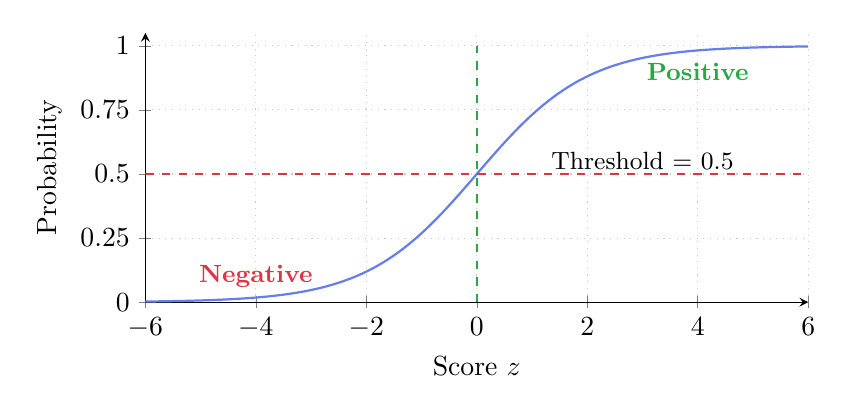
\begin{tikzpicture}
\begin{axis}[
  width=10cm, height=5cm,
  xlabel={Score $z$},
  ylabel={Probability},
  domain=-6:6,
  ymin=0, ymax=1.05,
  xmin=-6, xmax=6,
  xtick={-6,-4,-2,0,2,4,6},
  ytick={0,0.25,0.5,0.75,1.0},
  grid=major,
  grid style={dotted, gray!40},
  axis lines=left,
]
\addplot[thick, color=primary, samples=200] {1/(1+exp(-x))};
\addplot[dashed, color=negative, thick] coordinates {(-6,0.5)(6,0.5)};
\addplot[dashed, color=positive, thick] coordinates {(0,0)(0,1)};
\node at (axis cs:3, 0.55) {\small Threshold = 0.5};
\node[color=positive] at (axis cs:4, 0.9) {\small \textbf{Positive}};
\node[color=negative] at (axis cs:-4, 0.1) {\small \textbf{Negative}};
\end{axis}
\end{tikzpicture}
\caption{The sigmoid function maps any score to a probability between 0 and 1.}
\end{figure}

\begin{itemize}
  \item If $z$ is very large (positive) → probability $\approx 1.0$ → predict \textcolor{positive}{\textbf{positive}}
  \item If $z$ is very negative → probability $\approx 0.0$ → predict \textcolor{negative}{\textbf{negative}}
  \item If $z = 0$ → probability $= 0.5$ → \emph{uncertain}
  \item \textbf{Decision threshold}: If probability $> 0.5$, predict positive; otherwise, negative
\end{itemize}

\subsubsection{How the Model Learns — Training}

The model is trained by \textbf{minimising the loss function} (cross-entropy loss):

\[
\mathcal{L} = -\frac{1}{N} \sum_{i=1}^{N} \left[ y_i \log(\hat{p}_i) + (1 - y_i) \log(1 - \hat{p}_i) \right]
\]

where $y_i \in \{0, 1\}$ is the true label and $\hat{p}_i$ is the predicted probability. The \textbf{lbfgs solver} (a gradient-based optimisation algorithm) adjusts all 50{,}000 weights to minimise this loss.

\subsubsection{Regularisation — Preventing Overfitting}

The hyperparameter $C = 5$ controls \textbf{regularisation strength}:

\begin{itemize}
  \item \textbf{Overfitting}: Model memorises training data instead of learning general patterns
  \item \textbf{Regularisation}: Penalises very large weights, forcing the model to spread its reliance across many features rather than over-relying on a few
  \item $C = 5$ is a moderate setting — strong enough to generalise but not so strong as to underfit
\end{itemize}

\subsection{Train/Test Split}

\begin{conceptbox}[Train-Test Split]
We split the dataset into two parts:
\begin{itemize}
  \item \textbf{Training set (80\% = 40{,}000 reviews)}: The model learns from these. Weights are adjusted using this data.
  \item \textbf{Test set (20\% = 10{,}000 reviews)}: The model \emph{never sees} these during training. We use them to measure real-world performance.
\end{itemize}

\textbf{Why?} If we tested on the same data we trained on, the model could just memorise all the answers and get 100\% accuracy. The test set simulates how the model performs on \emph{new, unseen reviews} — the real use case.

\medskip
\textbf{Stratified split}: We ensure the 80/20 split maintains the 50/50 class balance in both sets.
\end{conceptbox}

\newpage

% ═════════════════════════════════════════════════════════════
\section{Model Evaluation Metrics}
% ═════════════════════════════════════════════════════════════

\subsection{Why Multiple Metrics?}

Accuracy alone can be misleading. Consider a disease that affects 1\% of people: a model that says ``no disease'' for everyone would have 99\% accuracy but be completely useless. We need more nuanced metrics.

\subsection{Confusion Matrix}

\begin{keyterm}{Confusion Matrix}
A confusion matrix shows all four possible outcomes of binary classification:

\medskip
\begin{center}
\begin{tabular}{r|cc}
 & \textbf{Predicted Positive} & \textbf{Predicted Negative} \\
\hline
\textbf{Actually Positive} & True Positive (TP) & False Negative (FN) \\
\textbf{Actually Negative} & False Positive (FP) & True Negative (TN) \\
\end{tabular}
\end{center}

\medskip
\begin{itemize}
  \item \textbf{TP}: Model said ``positive'', review was truly positive ✓
  \item \textbf{TN}: Model said ``negative'', review was truly negative ✓
  \item \textbf{FP}: Model said ``positive'', but review was actually negative ✗ (Type I error)
  \item \textbf{FN}: Model said ``negative'', but review was actually positive ✗ (Type II error)
\end{itemize}
\end{keyterm}

\subsection{Key Metrics Explained}

\subsubsection{Accuracy}

\[
\text{Accuracy} = \frac{TP + TN}{TP + TN + FP + FN}
\]

The fraction of all predictions that were correct. With our balanced dataset, this is a fair overall measure.

\subsubsection{Precision}

\[
\text{Precision} = \frac{TP}{TP + FP}
\]

Of all reviews the model labelled as positive, what fraction were \emph{actually} positive? High precision means few false alarms.

\subsubsection{Recall (Sensitivity)}

\[
\text{Recall} = \frac{TP}{TP + FN}
\]

Of all reviews that were \emph{truly} positive, what fraction did the model correctly identify? High recall means few missed positives.

\subsubsection{F1 Score}

\[
F_1 = 2 \times \frac{\text{Precision} \times \text{Recall}}{\text{Precision} + \text{Recall}}
\]

The F1 score is the \textbf{harmonic mean} of precision and recall. It provides a single balanced measure when both are important. An F1 of 1.0 is perfect; 0.0 is worst.

\subsubsection{ROC-AUC}

\begin{conceptbox}[ROC-AUC]
\textbf{ROC} = Receiver Operating Characteristic curve.
\textbf{AUC} = Area Under the Curve.

\medskip
The ROC curve plots the \emph{True Positive Rate} (recall) vs the \emph{False Positive Rate} at various classification thresholds. AUC measures the area under this curve:
\begin{itemize}
  \item AUC = 1.0 → Perfect classifier
  \item AUC = 0.5 → Random guessing (no better than a coin flip)
  \item AUC = 0.0 → Perfectly wrong (worse than random)
\end{itemize}

\textbf{AUC is threshold-independent}: It measures the model's discriminating ability regardless of where you set the positive/negative threshold.

\medskip
\textbf{Our model achieves AUC $\approx$ 0.98}, meaning it correctly ranks a randomly chosen positive review above a randomly chosen negative review 98\% of the time.
\end{conceptbox}

\subsection{Summary of Results}

\begin{center}
\begin{tabular}{lll}
\toprule
\textbf{Metric} & \textbf{Value} & \textbf{Interpretation} \\
\midrule
Accuracy  & $\sim$89--91\% & About 9 in 10 reviews correctly classified \\
F1 (Positive) & $\sim$0.90 & Excellent balance of precision \& recall for positive \\
F1 (Negative) & $\sim$0.90 & Excellent balance of precision \& recall for negative \\
ROC-AUC   & $\sim$0.97--0.98 & Near-perfect ranking ability \\
\bottomrule
\end{tabular}
\end{center}

\begin{whybox}
These results are competitive with state-of-the-art results on this dataset using simple models. The combination of careful text cleaning, TF-IDF with bigrams, and logistic regression is a powerful baseline that is fast to train and easy to deploy.
\end{whybox}

\newpage

% ═════════════════════════════════════════════════════════════
\section{The Streamlit Web Application}
% ═════════════════════════════════════════════════════════════

\subsection{What is Streamlit?}

\textbf{Streamlit} is a Python library that allows data scientists to create interactive web applications with only Python code — no HTML, JavaScript, or web development knowledge required. You write Python, and Streamlit renders it as a web page.

\subsection{Application Structure}

The app is organised into \textbf{5 tabs}, each corresponding to a stage of the pipeline:

\begin{center}
\begin{tikzpicture}[
  tab/.style={rectangle, rounded corners=4pt, draw=primary!60, fill=primary!12,
              minimum width=2.4cm, minimum height=1cm, font=\small, align=center},
]
  \node[tab] at (0,0)   {\faDatabase \\ \small Data Overview};
  \node[tab] at (2.8,0) {\faFilter \\ \small Data Cleaning};
  \node[tab] at (5.6,0) {\faChartBar \\ \small Visualisations};
  \node[tab] at (8.4,0) {\faRobot \\ \small Model \& Metrics};
  \node[tab] at (11.2,0){\faMagic \\ \small Live Prediction};
\end{tikzpicture}
\end{center}

\subsubsection{Tab 1 — Data Overview}

Displays dataset statistics and sample rows from the cleaned dataset. Uses \texttt{@st.cache\_resource} to load data efficiently. Shows 4 key metrics in styled cards: total reviews, average word count, maximum word count, and positive review count.

\subsubsection{Tab 2 — Data Cleaning}

Explains the 7-step cleaning pipeline with collapsible expanders. Shows before/after examples of 3 random reviews so users can see the transformation in action.

\subsubsection{Tab 3 — Visualisations}

Displays 5 pre-generated plots:
\begin{itemize}
  \item \textbf{Class distribution} — bar chart confirming the balanced 25k/25k split
  \item \textbf{Review length distribution} — histogram showing positive reviews tend to be slightly longer
  \item \textbf{Word clouds} — visual representations of the most frequent words in each class
  \item \textbf{Top 20 words per class} — bar charts showing the strongest discriminating words
\end{itemize}

\subsubsection{Tab 4 — Model \& Metrics}

Displays:
\begin{itemize}
  \item Model architecture table
  \item 4 metric cards (accuracy, F1 positive, F1 negative, ROC-AUC)
  \item Confusion matrix image
  \item ROC curve image
  \item Interactive styled classification report table
\end{itemize}

\subsubsection{Tab 5 — Live Prediction}

The most interactive tab. Has two modes:

\paragraph{Single Review Analysis:}
\begin{enumerate}
  \item User types/pastes a review into a text area
  \item Clicks ``Analyse Sentiment''
  \item App cleans the text using the same pipeline as training
  \item Transforms it to a TF-IDF vector
  \item Model predicts the sentiment and confidence
  \item Result is shown with colour-coded card (\textcolor{positive}{green} = positive, \textcolor{negative}{red} = negative)
  \item A \textbf{gauge chart} (Plotly) shows the probability of positive sentiment
  \item Cleaned text is shown in an expander for transparency
\end{enumerate}

\paragraph{Batch Prediction:}
\begin{enumerate}
  \item User enters multiple reviews (one per line)
  \item App processes all reviews at once
  \item Results shown in a colour-coded table
  \item Summary bar chart shows distribution of predictions
\end{enumerate}

\subsection{Key Technical Decisions in the App}

\subsubsection{@st.cache\_resource}

Loading a trained model from disk on every user interaction would be slow. The decorator \texttt{@st.cache\_resource} tells Streamlit to load the model \emph{once} and keep it in memory, reusing it for all subsequent requests. This is a critical optimisation.

\subsubsection{Gauge Chart for Confidence}

Instead of just showing ``89\% confident'', the app displays a gauge chart (like a speedometer). This is more intuitive — users can immediately see whether the prediction is strong (needle far left or far right) or uncertain (needle near the middle).

\subsubsection{Joblib for Model Persistence}

The trained model is saved to disk using \texttt{joblib.dump()} and loaded with \texttt{joblib.load()}. Three files are saved:
\begin{itemize}
  \item \texttt{tfidf\_vectorizer.joblib} — the fitted TF-IDF vectoriser (vocabulary + IDF scores)
  \item \texttt{logistic\_model.joblib} — the trained logistic regression model (weights)
  \item \texttt{meta.joblib} — metadata (accuracy, AUC, train size) for display in the sidebar
\end{itemize}

\newpage

% ═════════════════════════════════════════════════════════════
\section{The Complete Pipeline — End to End}
% ═════════════════════════════════════════════════════════════

\begin{figure}[H]
\centering
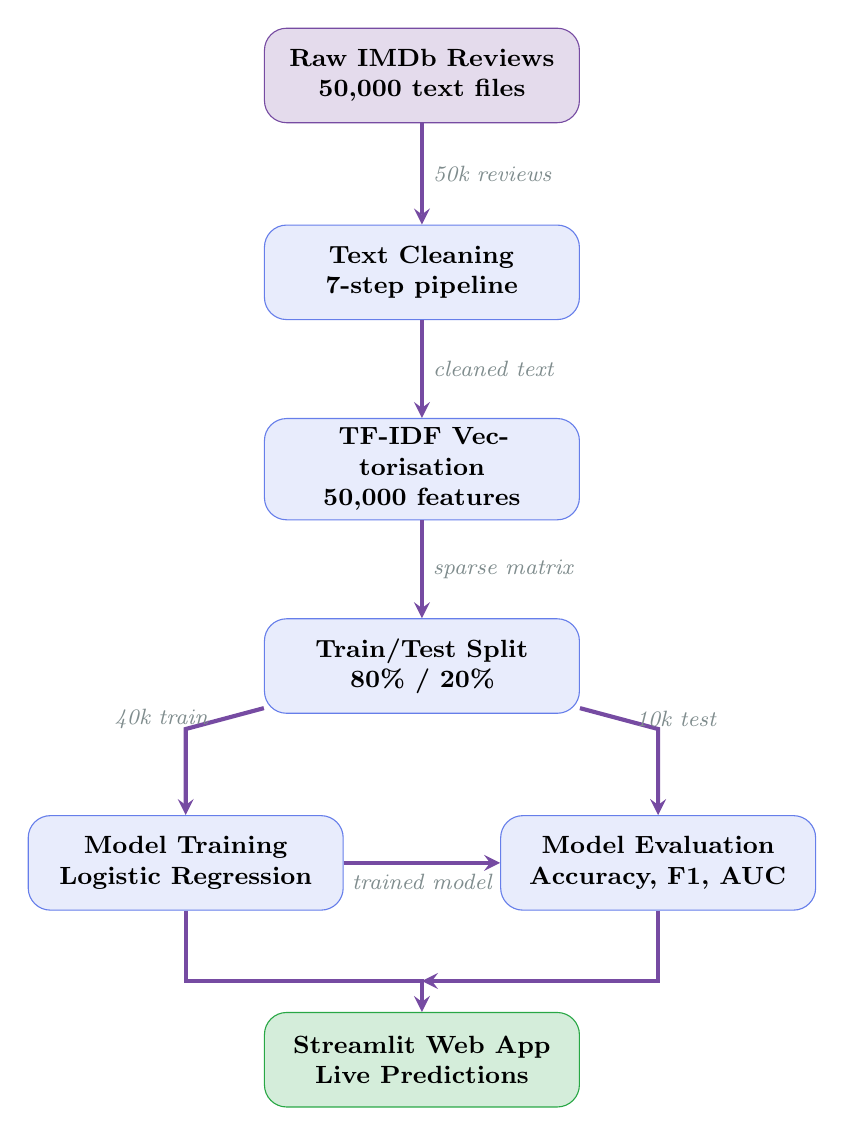
\begin{tikzpicture}[
  block/.style={rectangle, rounded corners=8pt, draw=primary, fill=primary!15,
                minimum width=4cm, minimum height=1.2cm, font=\small\bfseries, align=center,
                text width=3.5cm},
  arrow/.style={->, >=stealth, thick, color=secondary, line width=1.5pt},
  label/.style={font=\footnotesize\itshape, color=mutedtext},
]
  \node[block, fill=secondary!20, draw=secondary] (data)  at (0, 0)   {Raw IMDb Reviews \\ \small 50{,}000 text files};
  \node[block] (clean) at (0, -2.5)  {Text Cleaning \\ \small 7-step pipeline};
  \node[block] (tfidf) at (0, -5)    {TF-IDF Vectorisation \\ \small 50{,}000 features};
  \node[block] (split) at (0, -7.5)  {Train/Test Split \\ \small 80\% / 20\%};
  \node[block] (train) at (-3, -10)  {Model Training \\ \small Logistic Regression};
  \node[block] (eval)  at (3, -10)   {Model Evaluation \\ \small Accuracy, F1, AUC};
  \node[block, fill=positive!20, draw=positive] (app) at (0, -12.5) {Streamlit Web App \\ \small Live Predictions};
  
  \draw[arrow] (data)  -- node[label, right] {50k reviews} (clean);
  \draw[arrow] (clean) -- node[label, right] {cleaned text} (tfidf);
  \draw[arrow] (tfidf) -- node[label, right] {sparse matrix} (split);
  \draw[arrow] (split) -- node[label, left=2pt] {40k train} (-3, -8.3) -- (train);
  \draw[arrow] (split) -- node[label, right=2pt] {10k test} (3, -8.3) -- (eval);
  \draw[arrow] (train) -- node[label, below] {trained model} (eval);
  \draw[arrow] (train) -- (-3, -11.5) -- (0, -11.5) -- (app);
  \draw[arrow] (eval)  -- (3, -11.5)  -- (0, -11.5);
\end{tikzpicture}
\caption{Complete end-to-end sentiment analysis pipeline}
\end{figure}

\subsection{Training Script (\texttt{train\_pipeline.py})}

The training script (run separately before launching the app) performs:

\begin{enumerate}
  \item \textbf{Load data} — reads raw reviews from disk or HuggingFace Hub
  \item \textbf{Clean text} — applies the 7-step pipeline to all 50{,}000 reviews
  \item \textbf{Save cleaned CSV} — writes \texttt{data/reviews\_clean.csv} for the app's Data Overview tab
  \item \textbf{Generate visualisations} — creates all chart images and saves to \texttt{assets/}
  \item \textbf{TF-IDF vectorisation} — fits the vectoriser on training data only (prevents data leakage)
  \item \textbf{Train model} — fits logistic regression on training vectors
  \item \textbf{Evaluate} — computes all metrics on held-out test set
  \item \textbf{Save artifacts} — saves model, vectoriser, and metadata with joblib
\end{enumerate}

\begin{conceptbox}[Data Leakage]
\textbf{Data leakage} is a subtle but critical mistake: if you fit the TF-IDF vectoriser on the \emph{entire} dataset (including test data), the model gains unfair knowledge about the test set.

\medskip
\textbf{Correct approach (used here):}
\begin{enumerate}
  \item Split data into train and test \emph{first}
  \item Fit TF-IDF \textbf{only on training data}: learn vocabulary and IDF values from 40k reviews
  \item Transform \textbf{both} train and test using the fitted vectoriser
\end{enumerate}

This simulates the real-world scenario where the model encounters completely new text it has never seen.
\end{conceptbox}

\newpage

% ═════════════════════════════════════════════════════════════
\section{Visualisations — Understanding the Data}
% ═════════════════════════════════════════════════════════════

\subsection{Class Distribution}

A bar chart showing 25{,}000 positive and 25{,}000 negative reviews confirms the dataset is perfectly balanced. This is the first check any data scientist performs — imbalance here would require techniques like SMOTE or class-weight adjustment.

\subsection{Review Length Distribution}

A histogram of word counts (post-cleaning) for positive vs negative reviews. Research typically finds positive reviews are slightly longer — people tend to elaborate more on things they love. Negative reviews can be shorter and more direct (``Terrible film. Don't watch.'').

\subsection{Word Clouds}

A \textbf{word cloud} is a visual where words are displayed with size proportional to their frequency. It gives an immediate visual summary of the most common words in each class.

\begin{itemize}
  \item \textcolor{positive}{\textbf{Positive cloud}}: ``great'', ``love'', ``best'', ``wonderful'', ``brilliant'' dominate
  \item \textcolor{negative}{\textbf{Negative cloud}}: ``bad'', ``worst'', ``waste'', ``boring'', ``terrible'' dominate
\end{itemize}

These visualisations give us confidence that sentiment-bearing words exist in the data and that the classes are lexically separable.

\subsection{Top 20 Words per Class}

A bar chart showing the 20 most frequent words in positive vs negative reviews after cleaning. This confirms:
\begin{enumerate}
  \item Stopword removal worked (no ``the'', ``a'', ``is'')
  \item Clear lexical differences between classes exist
  \item The cleaning pipeline preserved meaningful sentiment words
\end{enumerate}

\newpage

% ═════════════════════════════════════════════════════════════
\section{Why This Approach Works — Strengths \& Limitations}
% ═════════════════════════════════════════════════════════════

\subsection{Strengths of TF-IDF + Logistic Regression}

\begin{itemize}
  \item \textbf{Speed}: Trains in seconds on 40{,}000 examples vs hours for deep learning
  \item \textbf{Interpretability}: You can inspect model weights to see which words most influence predictions
  \item \textbf{Low resource requirement}: Runs on a standard laptop without a GPU
  \item \textbf{Strong baseline}: Achieves $\sim$89--91\% accuracy, competitive with many deep learning approaches
  \item \textbf{No black box}: Every step is mathematically transparent
\end{itemize}

\subsection{Limitations}

\begin{itemize}
  \item \textbf{No word order}: ``I do not love this film'' and ``I love this film'' differ only by ``not'' — the model may misclassify the first as positive (though bigrams help)
  \item \textbf{No context}: The model cannot understand sarcasm (``Oh great, another boring sequel'')
  \item \textbf{Fixed vocabulary}: New words (slang, neologisms) not seen during training are unknown
  \item \textbf{No semantics}: The model does not know that ``magnificent'' and ``splendid'' mean similar things — they are treated as independent features
\end{itemize}

\subsection{How Modern Models Address These Limitations}

For production-grade sentiment analysis, transformer models like BERT, RoBERTa, or GPT are used because they:
\begin{itemize}
  \item Understand word context and order
  \item Handle negation and sarcasm better
  \item Use pre-trained semantic knowledge
\end{itemize}

However, they require significantly more computation and are harder to interpret. TF-IDF + Logistic Regression remains a powerful, practical choice for most real-world applications.

\newpage

% ═════════════════════════════════════════════════════════════
\section{Glossary of Key Terms}
% ═════════════════════════════════════════════════════════════

\begin{description}[style=nextline, leftmargin=2cm, labelwidth=1.8cm, font=\bfseries\color{primary}]

\item[NLP] Natural Language Processing — the field of AI focused on enabling computers to understand and process human language.

\item[Sentiment] The emotional tone of text — primarily positive, negative, or neutral.

\item[Corpus] A large collection of text documents used for NLP tasks. Our corpus = 50{,}000 IMDb reviews.

\item[Token] A single unit of text, usually a word. Tokenisation splits text into tokens.

\item[Stopwords] Extremely common words (``the'', ``a'', ``is'') that are usually removed in NLP because they carry little meaning.

\item[Lemmatisation] Converting words to their base dictionary form (``running'' → ``run'').

\item[Stemming] A cruder form of lemmatisation that chops word endings without a dictionary.

\item[N-gram] A sequence of $n$ consecutive words. Unigrams (n=1), bigrams (n=2), trigrams (n=3).

\item[TF-IDF] Term Frequency-Inverse Document Frequency. A numerical statistic that reflects how important a word is to a document in a collection.

\item[Feature] An individual measurable property or characteristic used as input to a model. Here, each TF-IDF value is a feature.

\item[Vectorisation] Converting text into numerical vectors that can be processed by ML algorithms.

\item[Sparse Matrix] A matrix where most values are zero. Our TF-IDF matrix is sparse because each review only uses a small fraction of the 50{,}000 vocabulary words.

\item[Logistic Regression] A classification algorithm that uses the sigmoid function to output probabilities.

\item[Sigmoid Function] A mathematical function that maps any real number to the range (0, 1), used to convert model scores to probabilities.

\item[Weights] The numerical parameters a model learns during training. Each feature has a weight.

\item[Overfitting] When a model performs well on training data but poorly on new data — it has memorised rather than learned.

\item[Regularisation] A technique to prevent overfitting by penalising large model weights.

\item[Train/Test Split] Dividing data into a training set (model learns from this) and test set (performance is measured on this).

\item[Accuracy] Fraction of all predictions that were correct.

\item[Precision] Of all predicted positives, what fraction are truly positive?

\item[Recall] Of all true positives, what fraction did the model find?

\item[F1 Score] Harmonic mean of precision and recall.

\item[ROC-AUC] Area Under the ROC Curve — measures the model's ability to discriminate between classes.

\item[Confusion Matrix] A table showing TP, TN, FP, FN counts for a classifier.

\item[Data Leakage] Contamination of the test set with information from training, leading to falsely optimistic evaluation.

\item[Joblib] A Python library for efficiently saving and loading Python objects (used to persist the trained model).

\item[Streamlit] A Python framework for rapidly building interactive data science web applications.

\item[Plotly] A Python library for creating interactive charts and visualisations.

\end{description}

% ═════════════════════════════════════════════════════════════
\section{Summary}
% ═════════════════════════════════════════════════════════════

This project demonstrates a complete, production-ready sentiment analysis pipeline. Starting from raw HTML-formatted IMDb movie reviews, it applies a 7-step text cleaning process, converts text to numerical TF-IDF features capturing both word-level and phrase-level patterns, and trains a logistic regression model to classify sentiment with approximately 90\% accuracy.

The Streamlit web application makes the entire pipeline accessible and interactive, from exploring the dataset and visualising word patterns, to evaluating the model and making live predictions on new text.

\medskip
The key takeaways are:

\begin{enumerate}
  \item \textbf{Text preprocessing is crucial}: Raw text is full of noise. Careful cleaning significantly improves model performance.
  \item \textbf{TF-IDF is powerful}: Simple word counts, properly weighted, capture most of the sentiment signal in text.
  \item \textbf{Logistic regression is underrated}: A well-tuned linear model often matches complex neural networks on text tasks.
  \item \textbf{Evaluation requires multiple metrics}: Accuracy alone is insufficient. Always examine precision, recall, F1, and AUC together.
  \item \textbf{Good engineering matters}: Caching, proper train/test splitting, and avoiding data leakage are as important as the model choice.
\end{enumerate}

\vfill
\begin{center}
\begin{tcolorbox}[colback=primary!10, colframe=primary, width=0.75\textwidth, arc=8pt]
\centering\small
\textbf{Built with:} Python $\cdot$ NLTK $\cdot$ scikit-learn $\cdot$ Streamlit $\cdot$ Plotly $\cdot$ Joblib \\[4pt]
\textbf{Dataset:} Stanford IMDb Large Movie Review Dataset \\[4pt]
\textbf{Algorithm:} TF-IDF (50k features, bigrams) + Logistic Regression (C=5)
\end{tcolorbox}
\end{center}

\end{document}